\documentclass{article}
\usepackage{graphicx}
\usepackage{tikz}

\begin{document}

\begin{figure}[h]
    \centering
    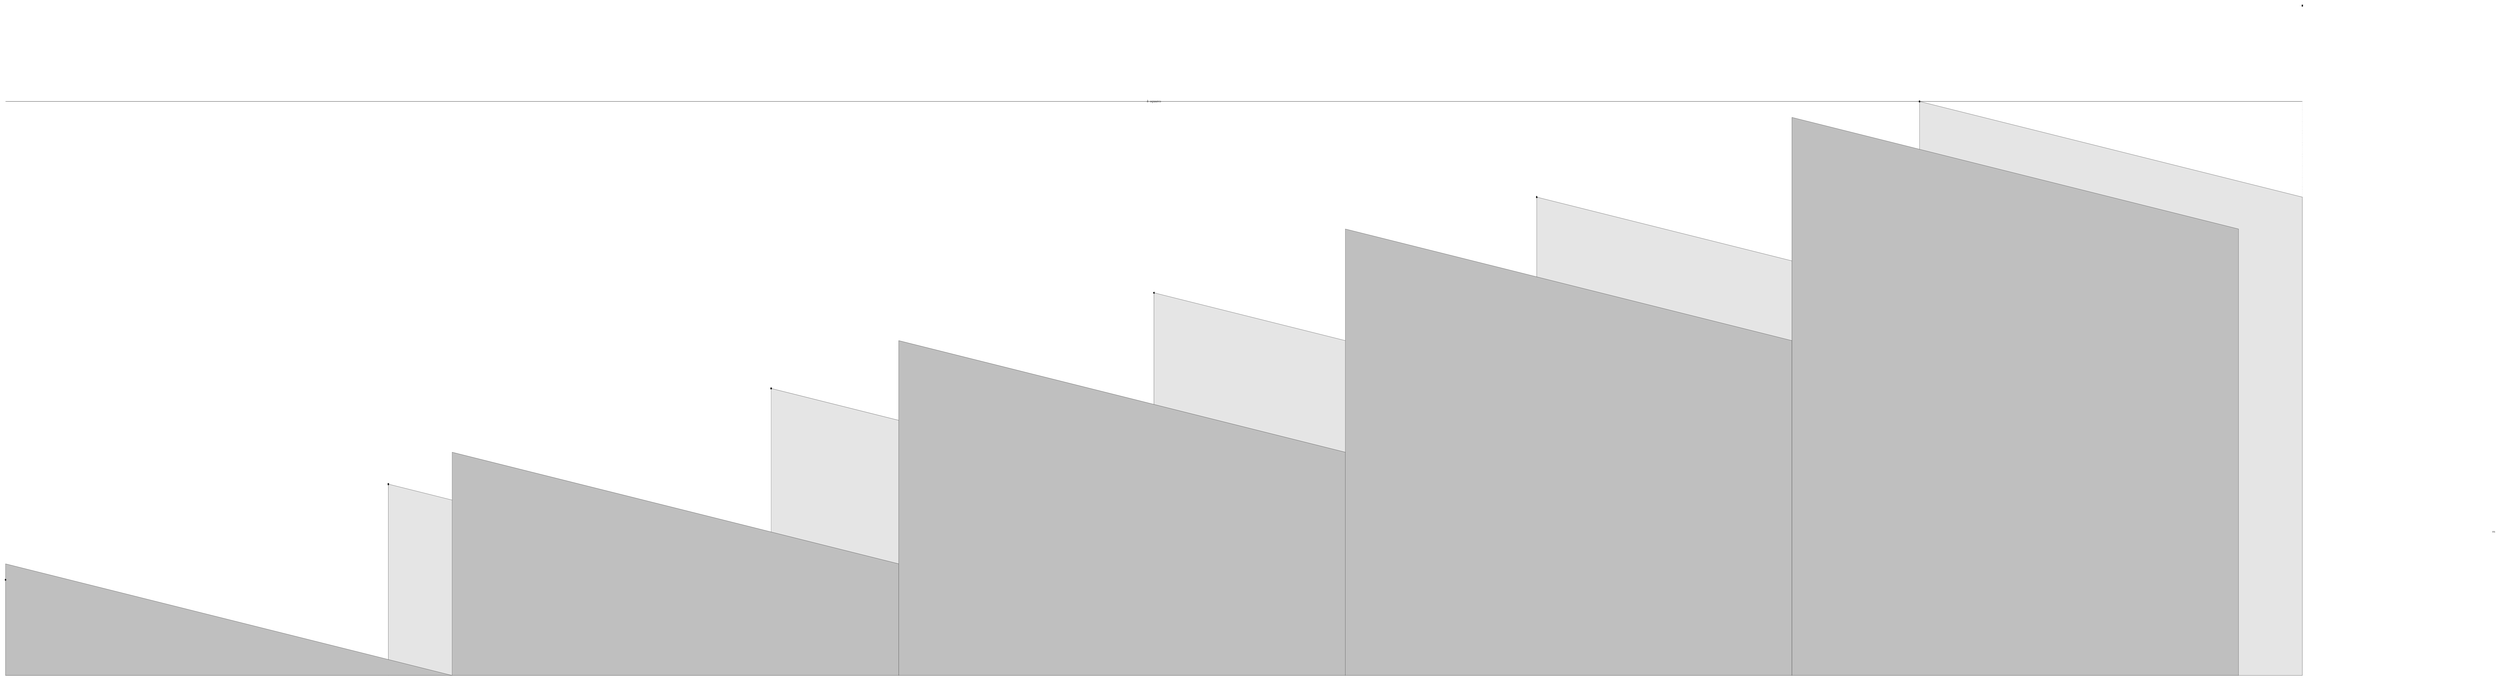
\begin{tikzpicture}[scale=0.75]
        % Draw the outer squares
        \foreach \i in {1,...,6} {
            \draw[fill=gray!20] ({(\i-1)*360/7},0) -- ({\i*360/7},0) -- ({\i*360/7},{(\i-1)*90/7}) -- ({(\i-1)*360/7},{\i*90/7}) -- cycle;
        }
        
        % Draw the inner squares
        \foreach \i in {1,...,5} {
            \draw[fill=gray!50] ({(\i-1)*360/6},0) -- ({\i*360/6},0) -- ({\i*360/6},{(\i-1)*90/6}) -- ({(\i-1)*360/6},{\i*90/6}) -- cycle;
        }
        
        % Draw the vertices
        \foreach \i in {1,...,7} {
            \node[circle, fill, inner sep=1.5pt] at ({(\i-1)*360/7},{\i*90/7}) {};
            \node at ({(\i-1)*360/7},{\i*90/7}) {\i};
        }
        
        % Draw the connecting lines
        \draw ({0*360/7},{6*90/7}) -- ({6*360/7},{6*90/7});
        
        % Label the length of the rectangle
        \node at ({3*360/7},{6*90/7}) {$k$ squares};
        
        % Draw the dotted line
        \draw[dotted] ({6*360/7},{6*90/7}) -- ({6*360/7},{1*90/7});
        
        % Draw the triangle
        \draw[fill=gray] ({6*360/7},{1*90/7}) -- ({6*360/7},{2*90/7}) -- ({6*360/7},{3*90/7}) -- cycle;
        \node at ({6.5*360/7},{1.5*90/7}) {$m$};
        
        \end{tikzpicture}
    \caption{A family of circlets $C(k,m)$. Let $k \geq 3$ and let $m \geq 4$ be even. To construct the 2-circlet $C(k,m)$, begin with the 2-complex illustrated here, whose 1-skeleton is the graph Cartesian product $K_{1,m}\Box P_{k+1}$. Identify the left $K_{1,m}$ with the right $K_{1,m}$ by a twist of $2\pi/m$, as indicated. The result is a {\it finned} 2-complex with a $C_{km}$ boundary. Cap this boundary by a polygon with $km$ sides. The result is a 2-circlet, as the $km$-gon shares an edge of degree 2 with any square, so any even $n$-subcomplex that contains the $km$-gon necessarily contains all the squares too.}
    \label{fig:CircletConstruction}
\end{figure}

\end{document}